%%%%%%%%%%%%%%%%%%%%%%%%%%%%%%%%%%%%%%%%%%%%%%%%%%%%%
% REPORT FOR SWISS-SEP 3.0 DATA ANALYSIS
%%%%%%%%%%%%%%%%%%%%%%%%%%%%%%%%%%%%%%%%%%%%%%%%%%%%%

% LATEX settings
\documentclass[a4paper, notitlepage, fleqn]{article} % USE titlepage IF YOU WANT TOC TO APPEAR ON NEXT PAGE
\usepackage[a4paper]{geometry}
\usepackage{stata} 

\usepackage[T1]{fontenc}
\usepackage[utf8]{inputenc}
 
\usepackage{fullpage} % SMALL MARGINS
% \usepackage[cm]{fullpage} % VERY SMALL MARGINS
 
\usepackage{lscape} % BETTER FOR PRINTING, PAGE DISPLAYED VERTICALLY
% \usepackage{pdflscape} % BETTER FOR SCREEN, PAGE DISPLAYED HORIZONTALLY
 
\usepackage{mathtools, amssymb, bookmark, framed, longtable, booktabs, graphicx, url, multirow, cancel}
 
\usepackage{hyperref}
\hypersetup{unicode=true, pdfborder = {0 0 0}, colorlinks, citecolor=blue, filecolor=black, linkcolor=blue, urlcolor=blue, pdftitle={Swiss-SEP 2.0 data analysis}, pdfauthor={Radoslaw Panczak}}

\renewcommand{\familydefault}{\sfdefault}
\usepackage[usenames, dvipsnames]{color}
\usepackage[table]{xcolor}
\usepackage[normalem]{ulem}

\usepackage[hang,flushmargin]{footmisc} 

% to avoid error http://tex.stackexchange.com/questions/165929/semiverbatim-with-tikz-in-beamer
\makeatletter
\global\let\tikz@ensure@dollar@catcode=\relax
\makeatother

\setlength{\parindent}{0pt} % no indent for ne paras
\graphicspath{ {d:/Data_RP/data/projects/EOLC/stata/graphres/} }
\setcounter{tocdepth}{2}

\usepackage{array}
\newcolumntype{L}[1]{>{\raggedright\let\newline\\\arraybackslash\hspace{0pt}}m{#1}}

% \linespread{1.3}
%
% \usepackage{setspace}
% \singlespacing
% \onehalfspacing
% \doublespacing

\usepackage{multirow}

% https://tex.stackexchange.com/questions/52317/pdftex-warning-version-allowed
\pdfminorversion=6

\title{\textbf{Swiss-SEP 2.0 index \endgraf 
Report 1.08 - data analysis}}

\author{Radoslaw Panczak \textit{et al.}}

\begin{document}

\maketitle
\tableofcontents

% %%%%%%%%%%%%%%%%%%%%%%%%%%%%%%%%%%%%%%%%%%%%%%%%%%%%%
% \newpage
% \section{Finding n'hoods with new buildings}
% %%%%%%%%%%%%%%%%%%%%%%%%%%%%%%%%%%%%%%%%%%%%%%%%%%%%%
\newpage
\section{PCA on n'hood aghgregated characteristics}
\begin{stlog}\input{log/ol_3.log.tex}\end{stlog}
% %%%%%%%%%%%%%%%%%%%%%%%%%%%%%%%%%%%%%%%%%%%%%%%%%%%%%
% \newpage
\section{Building age}

Construction period of the building is retrived sfrom \texttt{STATPOP 2018} dataset. Detailed typology is recoded to binary indicator flagging 
buildings constructed on or after 2001. Buidlings with missing information about age are treated as 'old' ones. 
\begin{stlog}\input{log/ol_6.log.tex}\end{stlog}
% %%%%%%%%%%%%%%%%%%%%%%%%%%%%%%%%%%%%%%%%%%%%%%%%%%%%%
\newpage
\section{Hybrid version of SEP}

This solution is mixing versions 1.0 \& 2.0. First the new buildings have value of index 1.0 assigned using the closest (linear dstance) neighbour. 

Then, construction period of the building is retrived sfrom \texttt{STATPOP 2018} dataset and then buildings built before year 2000 have the values of 1.0 index assigned and buildings constructed after 2000 have new values assigned. Buildings without the defined period of construction keep values 1.0 also. 
% %%%%%%%%%%%%%%%%%%%%%%%%%%%%%%%%%%%%%%%%%%%%%%%%%%%%%
\subsection{Index deciles}
\begin{stlog}\input{log/ol_8.log.tex}\end{stlog}
% %%%%%%%%%%%%%%%%%%%%%%%%%%%%%%%%%%%%%%%%%%%%%%%%%%%%%
\subsection{Quantiles}

Note that the original quantiles of second version :
\begin{stlog}\input{log/ol_9.log.tex}\end{stlog}
... are tad 'broken' after replacements:
\begin{stlog}\input{log/ol_10.log.tex}\end{stlog}
\begin{landscape}
Some transitions happened:  
\begin{stlog}\input{log/ol_11.log.tex}\end{stlog}
\end{landscape}

% %%%%%%%%%%%%%%%%%%%%%%%%%%%%%%%%%%%%%%%%%%%%%%%%%%%%%
\subsection{Bland Altman plots of diffs}

\begin{center}
\includegraphics[width=\textwidth]{gr/BA_sep1_sep2.png} 
\includegraphics[width=\textwidth]{gr/BA_sep1_sep3.png} 
\end{center}
% %%%%%%%%%%%%%%%%%%%%%%%%%%%%%%%%%%%%%%%%%%%%%%%%%%%%%
\newpage
\section{Maps}
\begin{center}
\includegraphics[width=\textwidth]{gr/sep-old.png} 
\includegraphics[width=\textwidth]{C:/projects/SNC_Swiss-SEP2/carto/01_sep-dots.png} 
\end{center}
% %%%%%%%%%%%%%%%%%%%%%%%%%%%%%%%%%%%%%%%%%%%%%%%%%%%%%
% %%%%%%%%%%%%%%%%%%%%%%%%%%%%%%%%%%%%%%%%%%%%%%%%%%%%%
\newpage
\section{Validation - SHP data}

% %%%%%%%%%%%%%%%%%%%%%%%%%%%%%%%%%%%%%%%%%%%%%%%%%%%%%
\subsection{Income graph - original}

\begin{center}
\includegraphics[width=.75\textwidth]{gr-orig/orig_income.png} 
\end{center}

% %%%%%%%%%%%%%%%%%%%%%%%%%%%%%%%%%%%%%%%%%%%%%%%%%%%%%
\subsection{Income graph - new indices}
\begin{center}
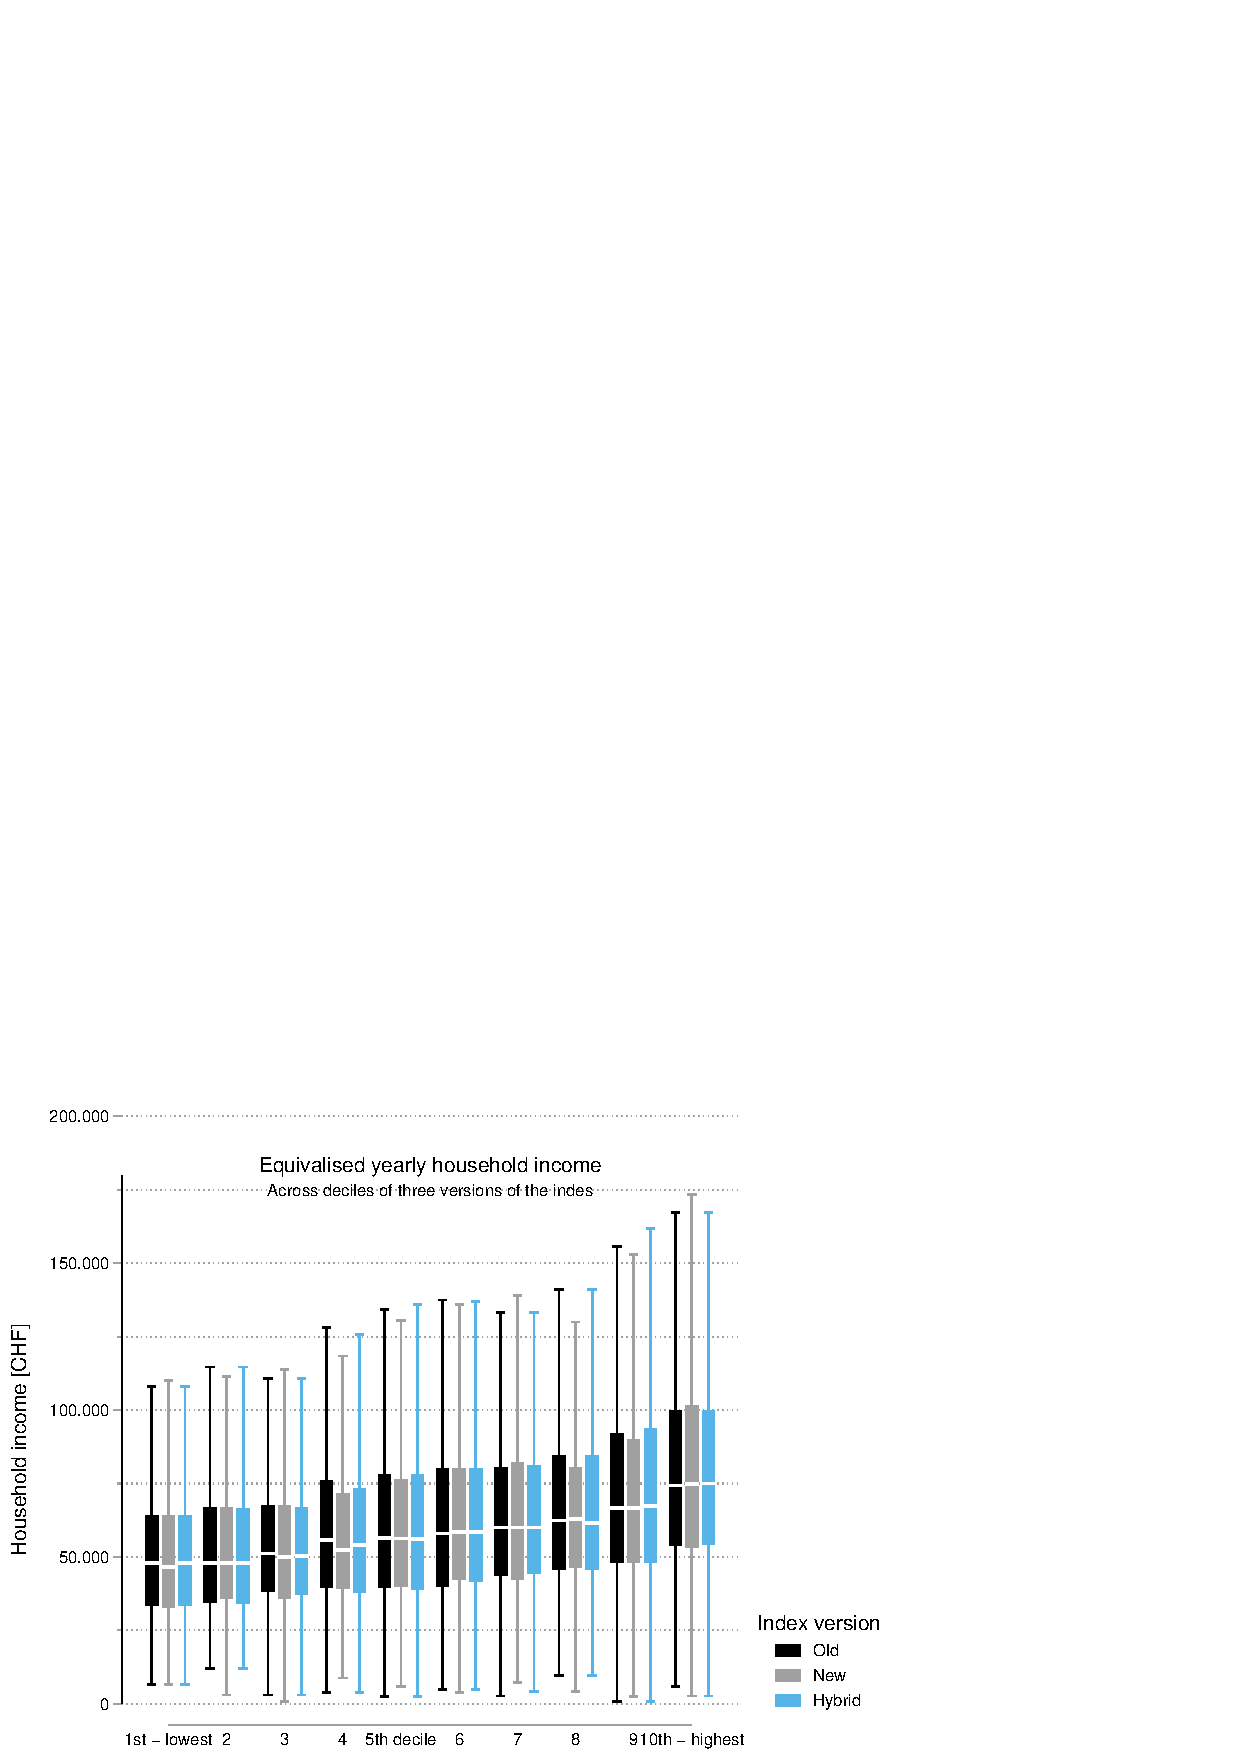
\includegraphics[width=.75\textwidth]{gr/shp_income.pdf} 
\end{center}

% %%%%%%%%%%%%%%%%%%%%%%%%%%%%%%%%%%%%%%%%%%%%%%%%%%%%%
\newpage
\subsection{Financial variables table - original}

\begin{center}
\includegraphics[width=.95\textwidth]{gr-orig/orig_shp_table.png} 
\end{center}

% %%%%%%%%%%%%%%%%%%%%%%%%%%%%%%%%%%%%%%%%%%%%%%%%%%%%%
\newpage
\subsection{Financial variables table - 1.0}
\begin{stlog}\input{log/ol_14.log.tex}\end{stlog}
\newpage
\begin{stlog}\input{log/ol_15.log.tex}\end{stlog}
\newpage
\begin{stlog}\input{log/ol_16.log.tex}\end{stlog}
% %%%%%%%%%%%%%%%%%%%%%%%%%%%%%%%%%%%%%%%%%%%%%%%%%%%%%
\newpage
\subsection{Financial variables table - 2.0}
\begin{stlog}\input{log/ol_17.log.tex}\end{stlog}
\newpage
\begin{stlog}\input{log/ol_18.log.tex}\end{stlog}
\newpage
\begin{stlog}\input{log/ol_19.log.tex}\end{stlog}
% %%%%%%%%%%%%%%%%%%%%%%%%%%%%%%%%%%%%%%%%%%%%%%%%%%%%%
\newpage
\subsection{Financial variables table - 3.0}
\begin{stlog}\input{log/ol_20.log.tex}\end{stlog}
\newpage
\begin{stlog}\input{log/ol_21.log.tex}\end{stlog}
\newpage
\begin{stlog}\input{log/ol_22.log.tex}\end{stlog}
% %%%%%%%%%%%%%%%%%%%%%%%%%%%%%%%%%%%%%%%%%%%%%%%%%%%%%
\newpage
\section{Validation - SNC mortality}

\subsection{All cause mortality - original}

\begin{center}
\includegraphics[width=.50\textwidth, angle = 270]{gr-orig/orig_hr_all.png} 
\end{center}

Note: 	Calculations from 'old' SNC data from the \textbf{2001 - 2008 period}, as described in original paper!

% %%%%%%%%%%%%%%%%%%%%%%%%%%%%%%%%%%%%%%%%%%%%%%%%%%%%%
\subsection{All cause mortality - new indices}
